\documentclass{beamer}
% example theorem blocks itemize \column{.45\textwidth} enumerate
\mode<presentation> {
\usetheme{Luebeck}%\usetheme{Madrid}
%\setbeamertemplate{footline} % To remove the footer line in all slides uncomment this line
%\setbeamertemplate{footline}[page number] % To replace the footer line in all slides with a simple slide count uncomment this line
%\setbeamertemplate{navigation symbols}{} % To remove the navigation symbols from the bottom of all slides uncomment this line
}
\usepackage{color}\usepackage{fancyvrb}\usepackage{listings}\usepackage{graphicx}\usepackage{booktabs}\usepackage{hyperref}
% Allows the use of \toprule, \midrule and \bottomrule in tables
\usepackage[style=verbose]{biblatex}
\bibliography{mp12}
\newcommand\verbbf[1]{\textcolor[rgb]{0,0,1}{\textbf{#1}}}
\definecolor{codegreen}{rgb}{0,0.6,0}\definecolor{codegray}{rgb}{0.5,0.5,0.5}\definecolor{codepurple}{rgb}{0.58,0,0.82}\definecolor{backcolour}{rgb}{0.95,0.95,0.92}
\lstdefinestyle{mystyle}{
    backgroundcolor=\color{backcolour},   
    commentstyle=\color{codegreen},
    keywordstyle=\color{magenta},
    numberstyle=\tiny\color{codegray},
    stringstyle=\color{codepurple},
    basicstyle=\footnotesize,
    breakatwhitespace=false,         
    breaklines=true,                 
    captionpos=b,                    
    keepspaces=true,                 
    %numbers=left,                    
    %numbersep=5pt,                  
    showspaces=false,                
    showstringspaces=false,
    showtabs=false,                  
    tabsize=1
}\lstset{style=mystyle}

%---------------------------------------------------------------------------------------------
\title[mp1\&mp2 experience share]{experience on mp1\&mp2} % The short title appears at the bottom of every slide, the full title is only on the title page
\author{Yihui He}
\institute[ ] % Your institution as it will appear on the bottom of every slide, may be shorthand to save space
{
   % Your institution for the title page
\medskip
\textit{yihuihe@foxmail.com}
}\date{\today}

\begin{document}
\begin{frame}
\titlepage
\end{frame}
\begin{frame}
\frametitle{Overview}
\tableofcontents
\end{frame}

%----------------------------------------------------------------------------------------
%	PRESENTATION SLIDES
%----------------------------------------------------------------------------------------

\section{mp1}
\begin{frame}
\frametitle{Goal}
\begin{columns}
\begin{column}{.5\textwidth}
\begin{itemize}
\item Input: CIFAR 10 image
\item Architecture: two-layer neural network
\item Output:prediction among 10 classes
\end{itemize}
\end{column}
\begin{column}{.45\textwidth}
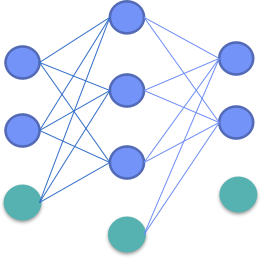
\includegraphics[width=\textwidth]{mp1.png}
\end{column}
\end{columns}



\end{frame}
%------------------------------------------------
\subsection{tricks}
%------------------------------------------------
\begin{frame}[fragile]
\frametitle{tuning hyperparameters}
\begin{itemize}
\item determine ralation\footnote{stanford cs231n} between parameter and backpropagation error:
linear, $\theta \propto \delta$ or exponential, $log(\theta)\propto \delta$
\item run a grid search(or random search) on a small part of our big dataset
\end{itemize}
\begin{lstlisting}[language=python]
for hidden_neurons in range(150,600,50):
  for learning_rate in [1e-3*10**i for i in range(-2,3)]:
    for norm in [0.5*10**i for i in range(-3,3)]:
      [loss_history,accuracy]=\
      train(small_dataset,
            hidden_neurons,learning_rate,norm)
      # dump loss, accuracy history for each setting
      # append highest accuracy of each setting to a .csv
\end{lstlisting}
\end{frame}

%------------------------------------------------
\begin{frame}
\frametitle{Choosing number of hidden neurons}
\begin{table}
\caption{top accuracy}
\begin{tabular}{|l|l|l|l|}
\hline
\multicolumn{1}{|p{1cm}|}{\centering hidden \\ neurons}
&\multicolumn{1}{|p{1cm}|}{\centering learning \\ rate}
&\multicolumn{1}{|p{2cm}|}{\centering regularization \\ strength}
&\multicolumn{1}{|p{1.5cm}|}{\centering validation \\ accuracy}\\
\hline
350 & 0.001    & 0.05   & 0.516 \\
\hline
400 & 0.001    & 0.005  & 0.509 \\
			\hline
250 & 0.001    & 0.0005 & 0.505 \\
			\hline
250 & 0.001    & 0.05   & 0.501 \\
			\hline
150 & 0.001    & 0.005  & 0.5   \\
			\hline
500 & 0.001    & 0.05   & 0.5  \\
\hline
\end{tabular}
\end{table}
\end{frame}

%------------------------------------------------
\begin{frame}
\frametitle{Update methods affect converge rate}
1000 iterations, batch size 100
\begin{table}
\centering
\caption{Differences between update methods}
\begin{tabular}{lllll}
accuracy & Train & Validation & Test &  \\
SGD      & .27   & .28        & .28  &  \\
Momentum & .49   & .472       & .458 &  \\
Nesterov & .471  & .452       & .461 &  \\
RMSprop  & .477  & .458       & .475 & 
\end{tabular}
\end{table}
These update methods can't make final accuracy higher(sometimes even lower than fine-tuned SGD),
 but make training much faster.
\end{frame}
%------------------------------------------------
\begin{frame}[fragile]
 \frametitle{dropout}
 Accuracy improves about 3\%. \\
 Only need to change one line in code:
\begin{lstlisting}[language=python]
a2=np.maximum(X.dot(W1)+b1,0)
a2*=(np.random.randn(*a2.shape)<p)/p #add this line
scores=a2.dot(W2)+b2
\end{lstlisting}
p  : dropout rate (usually choosen from .3 .5 .7) \\
a2 : activation in the second layer.
\end{frame}


\begin{frame}
\frametitle{initialization methods}
Three comment initialization for fully connected layer:
\begin{itemize}
\item $\text{N}(0,1)\sqrt{1/n}$
\item $\text{N}(0,1)\sqrt{2/(n_{in} + n _{out}})$ 
\item $\text{N}(0,1)\sqrt{2/n}$
\end{itemize}
Significance can't be seen from our two layers shallow neural net.\\
However, initialization is super important in mp2(deep neural net).
\end{frame}

\begin{frame}
\begin{huge}\centerline{questions about these tricks?}\end{huge}
\end{frame}
%------------------------------------------------
\subsection{new model}
\begin{frame}
\frametitle{new model}
After using tricks we mentioned, accuracy is around 55\%, 
neural network architecture is already fixed. \\
\phantom{dsf}
\begin{huge}
how do we improve accuracy?
\end{huge}
\end{frame}

\begin{frame}
\frametitle{algoritms leaderboard\footnote{rodrigob.github.io}}
At the very bottom of leaderboard(State-of-the-art is 96\%):
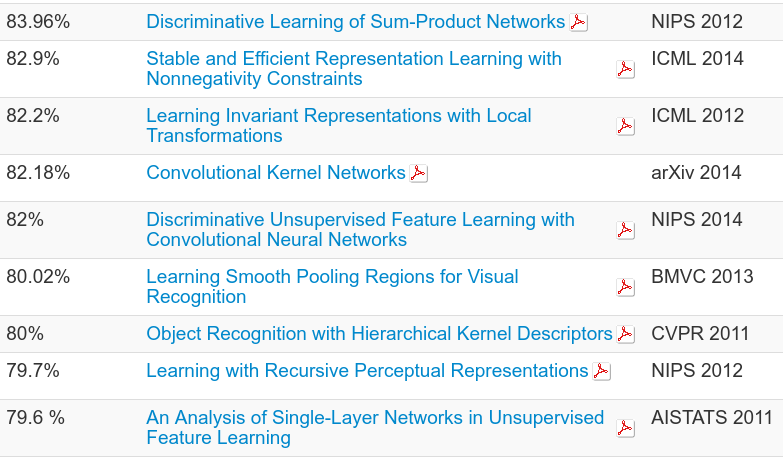
\includegraphics[width=\textwidth]{rank.png}
\end{frame}

\begin{frame}
\frametitle{preprocessing\footcite{coates2011analysis}}
The new model I used benefit from two preprocessing techniques:
\begin{enumerate}
 \item PCA whitening
 \item Kmeans
 \item plug in our two-layer neural network (the original paper use SVM at the end)
\end{enumerate}
\end{frame}
%------------------------------------------------
\begin{frame}
\frametitle{high level description}
Learn a feature representation:
\begin{enumerate}
\item Extract random patches from unlabeled training images.
\item Apply a pre-processing stage to the patches.
\item Learn a feature-mapping using an unsupervised learning algorithm.
\end{enumerate}
Given the learned feature mapping, we can then perform feature extraction:
\begin{enumerate}
\item Break an image into patches.
\item Cluster these patches. 
\item Concatenate cluster result of each patch \{0,0,...,1,...,0\}, as new representation of this image.
\end{enumerate}
\end{frame}
%------------------------------------------------
\begin{frame}
\frametitle{steps}
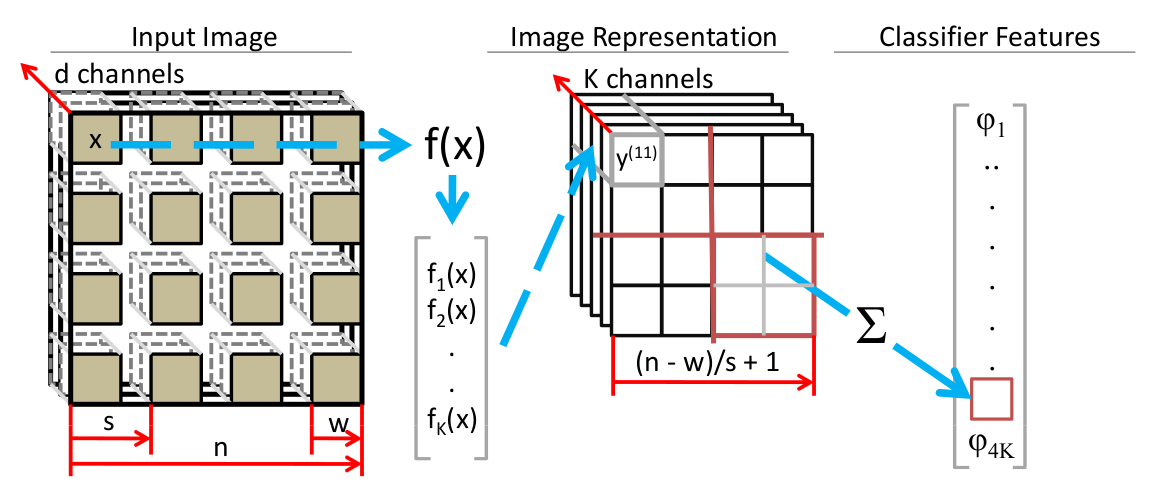
\includegraphics[width=\textwidth]{kmeans.png} 
\end{frame}
%------------------------------------------------
\begin{frame}
\frametitle{PCAwhitening visualize}
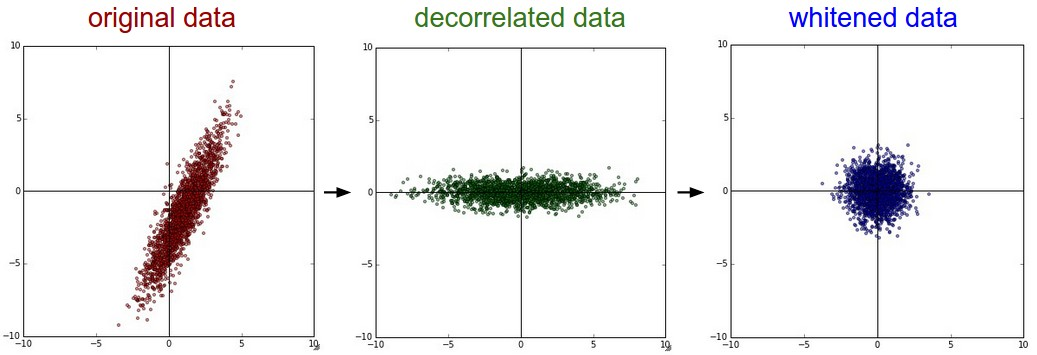
\includegraphics[width=\textwidth]{pca.jpeg}
Use PCAwhitening without dimention reduction.
\end{frame}
\begin{frame}
\frametitle{Kmeans visualize}
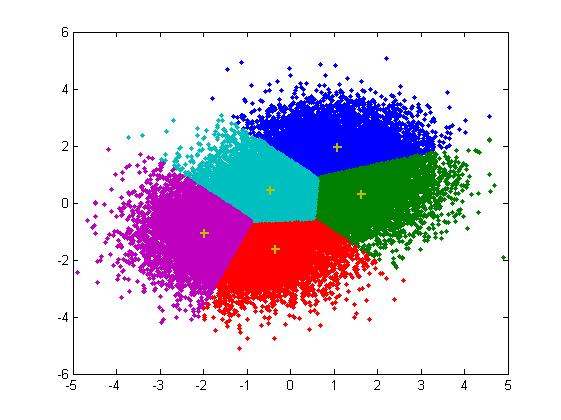
\includegraphics[width=.8\textwidth]{kmeans.jpg}\\
Select 1600 clusters
\end{frame}

%------------------------------------------------
\begin{frame}
\frametitle{PCAwhitening effect on Kmeans}
Some cluster centroids
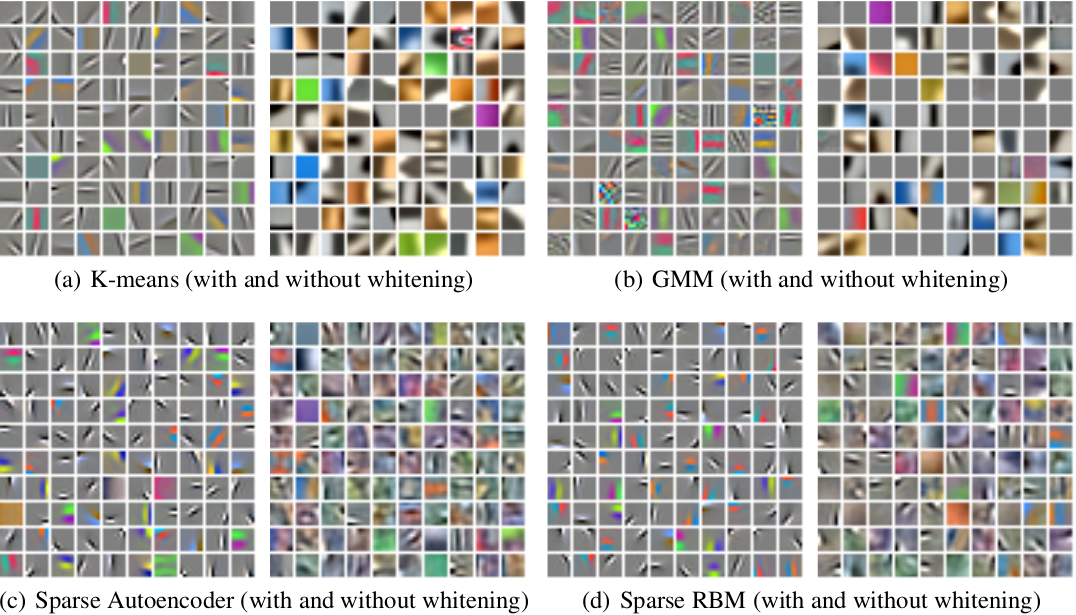
\includegraphics[width=\textwidth]{whiten.png}

\end{frame}
%------------------------------------------------
\begin{frame}
\frametitle{When should we stop training?}
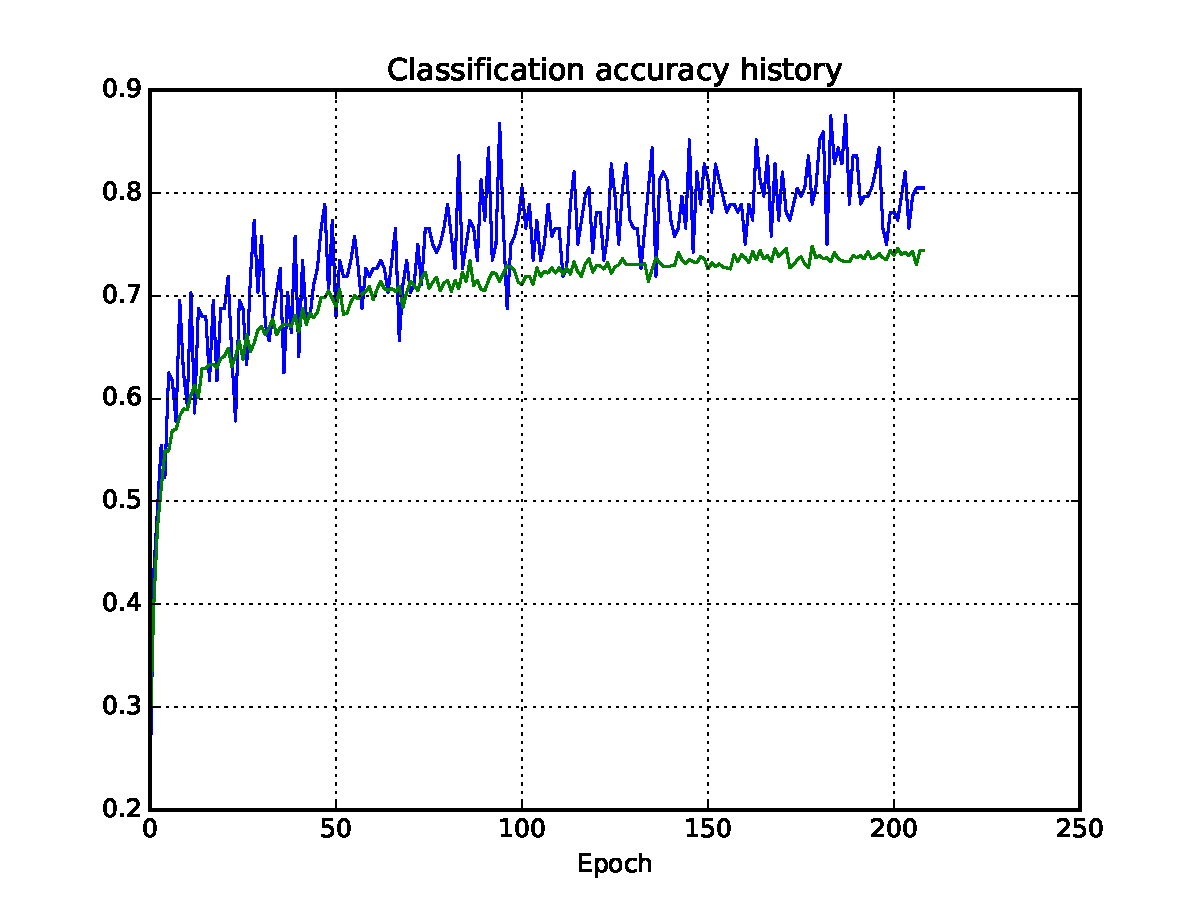
\includegraphics[width=.9\textwidth]{kmeans_acc-eps-converted-to.pdf}
\end{frame}

\begin{frame}
\frametitle{more information from results}
    \begin{table}
    	\centering
    	\begin{tabular}{lllll}
    	\toprule
				& Naive & Dropout & Preprocessed & \\
				\midrule
	  hidden nodes    & 350   & 500        & 200 & \\
	  learning rate & $1\times10^{-3}$   & $1\times10^{-4}$       & $5\times10^{-4}$ &  \\
	  learning rate Decay & .95   & .95       & .99 &  \\
	  regularization & L2,0.05  & Dropout,.5       & Dropout,.3 &  \\
	  Activation  & ReLU  & Leaky ReLU       & ReLU &  \\
	  Update method  & SGD  & Momentum,0.9       & Momentum,0.95   &  \\
	  Iterations & $1\times10^{4}$  & $1\times10^{4}$       & $7\times10^{4}$ &  \\    		
	  Batch size & 100  & 100       & 128 &  \\    		
	  Time(min)  & 15  & 80       & 110 &     		\\
	  Train accuracy  & 60\%  & 65\%       & 80\% & \\
			Validation  & 55\%  & 62\%       & 75\% &     	\\	
    		Test  & 52\%  & 55\%       & 74\% &     		
    	\end{tabular}
    \end{table}
\end{frame}

\begin{frame}
\frametitle{importance of mean image substraction}
The result I got is 75\%, the orignal paper get 79\%. \\
It's because I forgot to subtract mean before doing PCA whitening. 
After fix this bug, accuracy increases to 77\%. Much closer. \\ \phantom 
A Huge difference! Mean image substraction is important.
\end{frame}

\begin{frame}
\begin{huge}\centerline{questions on PCAwhitening and Kmeans?}\end{huge}
\end{frame}
\section{mp2}
%------------------------------------------------
\begin{frame}
\tableofcontents
\end{frame}


\begin{frame}
\frametitle{Goal}
\begin{itemize}
\item Input: CIFAR 100 image
\item Archtecture: Not determined
\item Output:prediction among 20 classes
\end{itemize}
\end{frame}

\subsection{tricks}
%------------------------------------------------
\begin{frame}
\frametitle{tricks that show little difference in my experiments}
\begin{itemize}
\item Dropout
\item Update methods
\item PCA whitening and Kmeans
\end{itemize}
\end{frame}


\begin{frame}
\frametitle{Initialization methods}
Becomes more and more important when network goes deep.\\
Recall that we have two problems: gradient vanishing $(\beta _w \beta _\alpha)^p\ll 1$ and gradient exploding $(\beta _w \beta _\alpha)^p\gg 1$: 
\begin{itemize}
\item Orthogonal initalization
\item LUSV initalization
\item Xavier initialization
\item Kaiming He\footcite{he2015delving} initialization method({\color{red}works best})
\end{itemize}
\end{frame}

\begin{frame}
\frametitle{Kaiming He's initialization method}
The idea is scale backward pass signal to 1 at each layer. Implementation is very simple.
\[std=sqrt(2/Depth_{in}/receptionFieldSize).\]
$Depth_{in}$: number of filters of previous layer comes in.\\
receptionFieldSize: eg. 3x3\\
\end{frame}
\begin{frame}
\frametitle{could to make 30 layers deep net converge}
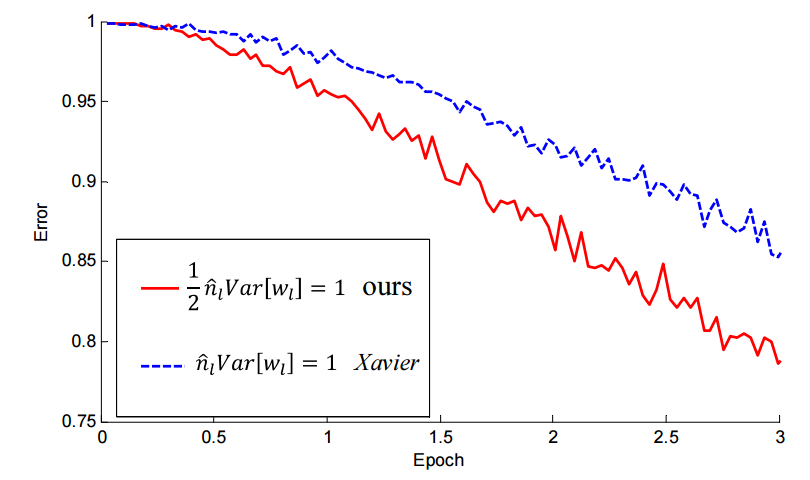
\includegraphics[width=\textwidth]{init.png}
\end{frame}

\begin{frame}
\frametitle{number of hidden neurons}
\begin{itemize}
\item More hidden neurons may not show any superior, only increasing time cost.
\item Adding hidden layers sometimes make things worse.\\
Kaiming He\footcite{he2015deep} found that about 30\% redundant computation comes from the fully connected layers. 
Fully connected layer is less efficient than conv layer.
\end{itemize}
One solution: replace the fully connected layer between the last conv layer and hidden layer with global average pooling.
\end{frame}
\subsection{choosing from different models}
\begin{frame}
\frametitle{New model}
How do we improve it?\\
To my knowledge, I found these possible way to improve accuracy:
\begin{itemize}
\item XNOR net\footcite{rastegari2016xnor}
\item mimic learning\footcite{ba2014deep} (model compression)
\item switch to faster framework(mxnet\footcite{chen2015mxnet}), rather than tensorflow :)
\item residual neural network\footcite{he2015deep}
\end{itemize}
\end{frame}


\begin{frame}
\frametitle{what is XNOR net?}
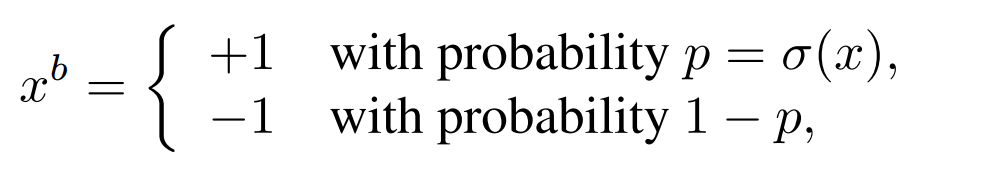
\includegraphics[width=\textwidth]{binary.png}\\
$\sigma(x)$, activation function
\end{frame}

\begin{frame}
\frametitle{XNOR net speed}
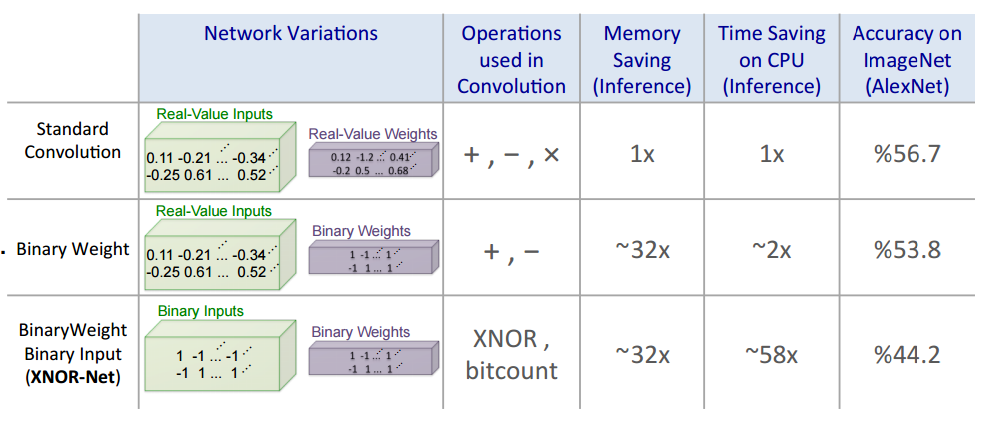
\includegraphics[width=\textwidth]{xnornet.png}\\
\begin{block}
{How fast is it?}
State-of-the-art neural net need 60 hours(200 epochs) to reach 95\% on CIFAR10 on my laptop. 
Using XNOR net, it will only spends 1 hour.
\end{block}
\end{frame}

\begin{frame}
\frametitle{deep learning framework comparison}
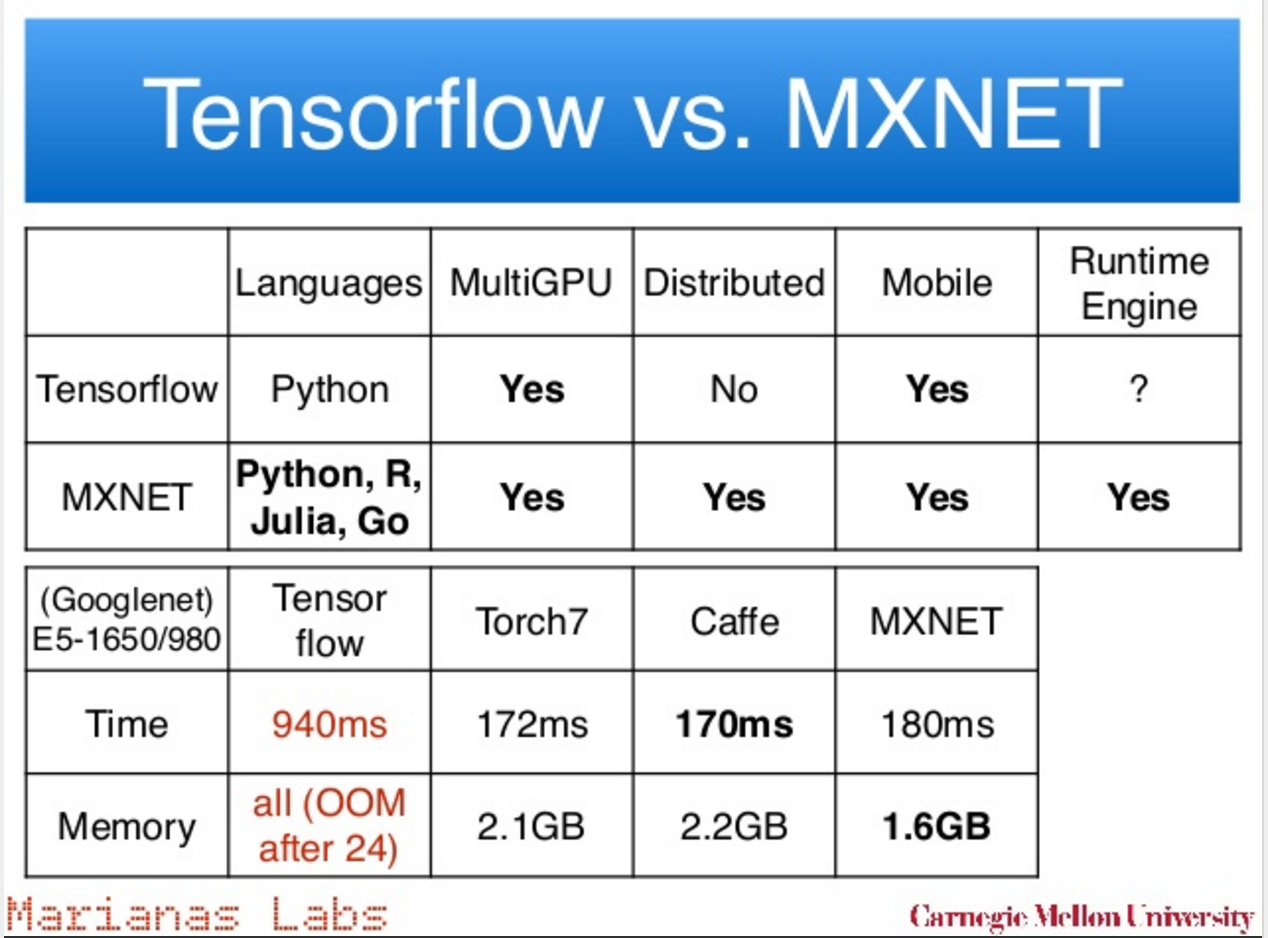
\includegraphics[width=.8\textwidth]{mxnet.png}
\end{frame}


\begin{frame}
\frametitle{what is mimic learning, basic idea}
With a high accuracy teacher model,\\
we not only tell the student neural network which label is true or wrong(0,1)\\
also tell the student neural network some classes are close to each other and some are not.\\
\begin{example}
In CIFAR10, truck and car are in different classes, however, they share some common features. So when there's a car in the image, truck's probability is also high. Teacher model helps student model jointly learn these two concepts.
\end{example}
\end{frame}

\begin{frame}
\frametitle{what is mimic learning, details}
High level overview:
\begin{enumerate}
\item train a state-of-the-art neural network
\item get the $log(p_{deep}(y|X))$ for training set
\item replace the softmax layer of shallow neural network with a linear regressor
\item minimize log probability error: $J(\theta)=\sum_{y\in labels}(log(p(y|X))-log(p_{deep}(y|X)))^2$
\item put back softmax layer
\item fine tuning
\end{enumerate}
\end{frame}


\begin{frame}
\frametitle{result from paper}
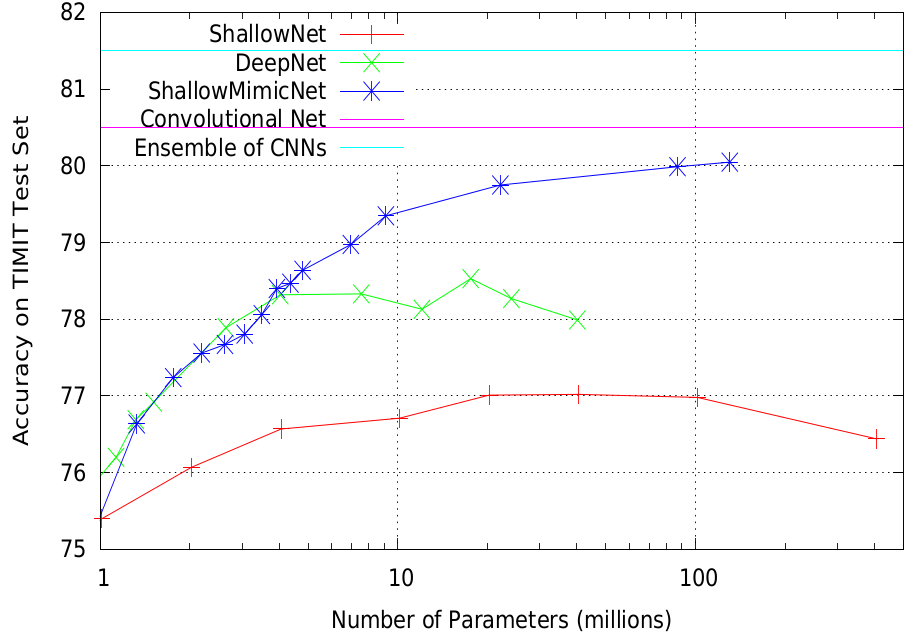
\includegraphics[width=.8\textwidth]{mimic.png}
\end{frame}

\begin{frame}
\frametitle{residual neural network}
Basic idea:\\
Learn $f(x)-x$ instead of $f(x)$.
\end{frame}
%--------------------------------------------------------------
\subsection{delving into one model}


\begin{frame}
\frametitle{residual neural network}
The only two differences between residual neural network and ConvNet:
\begin{enumerate}
\item no hidden layers
\item use shortcut module, which allows a layer skip the layer on top of it,
 and pass its value to the next layer.
\end{enumerate}
\end{frame}

\begin{frame}
\begin{columns}
\begin{column}{.1\textwidth}
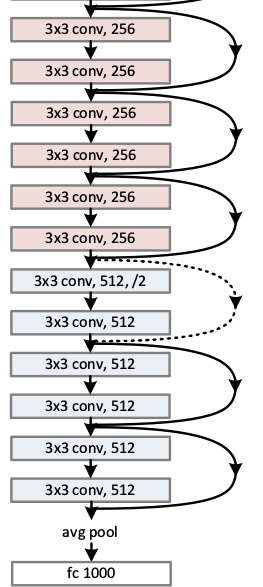
\includegraphics[scale=.35]{resArch.png}
\end{column}
\begin{column}{.5\textwidth}
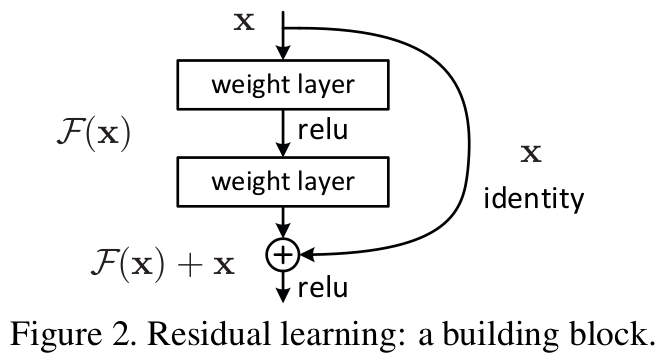
\includegraphics[width=1.3\textwidth]{resnet.png}
\end{column}
\end{columns}
\end{frame}


\begin{frame}
\frametitle{traditional convolutional neural network}
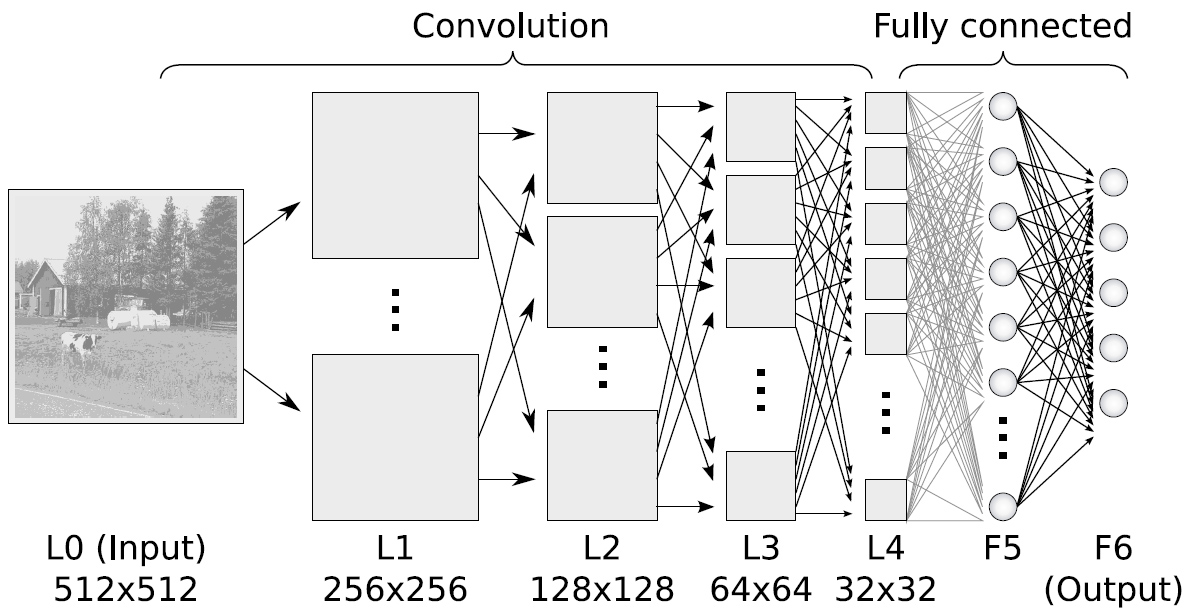
\includegraphics[width=\textwidth]{Alex.jpg}
\end{frame}


\begin{frame}[fragile]
\frametitle{parameters on each layers}
\begin{columns}
\begin{column}{.5\textwidth}
 A commonly used VGGnet:
\begin{verbatim}
 conv3-64  x 2 : 38,720
 conv3-128 x 2 : 221,440
 conv3-256 x 3 : 1,475,328
 conv3-512 x 3 : 5,899,776
 conv3-512 x 3 : 7,079,424
 fc1           : 102,764,544
 fc2           : 16,781,312
 fc3           : 4,097,000
 TOTAL         : 138,357,544
\end{verbatim}
\end{column}
\begin{column}{.5\textwidth}
Notice that 74\% parameters are from fc1, however, actual accuracy improvement is from conv layers. Residual nerual network, instead, uses all convolution layers
 and a global average pooling layer at the end.
\end{column}
\end{columns}
{\color{white}{ a}}\\
{\color{white}{ a}}\\
\cite{springenberg2014striving},
\end{frame}


\begin{frame}
\frametitle{architecture comparison}
  \begin{table}[!hbt]
  \centering
  \caption{Differences between three archectures}
  \begin{tabular}{lllll}
  & AlexNet & Kmeans & ResNet & \\
  parameters    & 1M   & .4M & .13M & \\
  Layers      & 7 & 3 & 14 \\
  learning rate & $.1$   & $5\times10^{-4}$ & $.1$ &  \\  
  regularization & L2  & Dropout,.3       & None &  \\
  epoch & 10  & 140       & 18 &  \\    		
  Batch size & 128  & 128       & 256 &  \\    		
  Time(min)  & 180  & 80       & 180 &\\
  CIFAR10 Acc & 82\% & 75\% & 84\% \\
  Train accuracy  & 90\%  & 80\%       & 86\% & \\
  Test  & 56\%  & 56\%       & 63\% &     		
  \end{tabular}
  \end{table}

\end{frame}

\begin{frame}
\frametitle{why residual neural network more efficient?}
\begin{enumerate}
\item Less trainable parameters than neural networks that have the same depth.
\item Lower layer response.
\item shortcut module allows error $\delta$ directly pass to previous layers, 
instead of going through each layer. 
It implicitly makes a deeper network shallower, so it won't suffer much from gradient vanishing and exploding.
It makes training faster.
\end{enumerate}
\end{frame}

\begin{frame}
Code, report and papers can be access via github:\\
mp1\\
\href{https://github.com/yihui-he/Single-Layer-neural-network-with-PCAwhitening-Kmeans}{https://github.com/yihui-he/Single-Layer-neural-network-with-PCAwhitening-Kmeans}\\
mp2\\
\href{https://github.com/yihui-he/Residual-neural-network}{https://github.com/yihui-he/Residual-neural-network}
\end{frame}

\begin{frame}
\Huge{\centerline{questions?}}
\end{frame}
%----------------------------------------------------------------------------------------

\end{document}